\section*{Ziele}
\begin{frame}
\frametitle{Lernziele}
Am Ende des Semesters können Sie
\begin{itemize}
\item die Grundbegriffe der Statistik unterscheiden und erläutern,
\pause
\item grundlegende statistische und wahrscheinlichkeitstheoretische Kennzahlen bestimmen und interpretieren,
\pause
\item ausgewählte maschinelle Lernverfahren in ihren Grundzügen erklären und einsetzen,
\pause
\item Aufgabentypen des maschinellen Lernens unterscheiden und für den jeweiligen Aufgabentyp geeignete Verfahren benennen,
\pause
\item erlernte Modelle validieren und testen,
\pause
\item Ergebnisse der Datenanalyse visualisieren,
\pause
\item die Anforderungen an ein Datenbanksystem benennen und erläutern.
\end{itemize}
\end{frame}
%\begin{frame}
%\frametitle{Der rote Faden}
%% Für Bilder Argument T benutzen:
%    \begin{columns}[T]
%        \begin{column}{0.49\textwidth}
%            \begin{itemize}%[<+->] Kommentar entfernen falls jeder Punkt einzeln erscheinen soll
%            	\item[$\,\blacktriangleright$] Daten aufnehmen
%            	\begin{itemize}
%            		\item Was sind Daten?
%            		\item Woher kommen Daten?
%            	\end{itemize}	
%            	\item[$\,\blacktriangleright$] Daten speichern
%            		\begin{itemize}
%            			\item Welche Anforderungen gibt es an Datenbanken?
%            			\item Wie kann ich Daten in einer relationalen Datenbank abrufen?
%            		\end{itemize}
%            	\item[$\,\blacktriangleright$] Daten auswerten
%            	\begin{itemize}
%            		\item Welche Möglichkeiten zur Auswertung gibt es?
%            		\item Was ist maschinelles Lernen und was sind die Einsatzmöglichkeiten?
%            		\item Wie prüfe ich ein erlerntes Modell?
%            		\item Wie kann ich Ergebnisse visualisieren?
%            	\end{itemize}
%        	\end{itemize}
%        \end{column}
%        \begin{column}{0.49\textwidth}
%            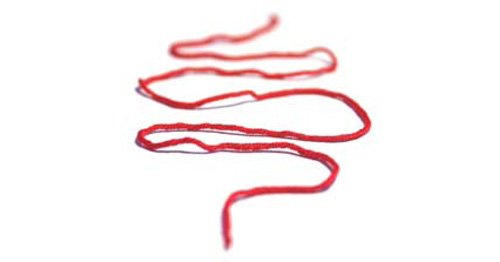
\includegraphics[width=\textwidth]{images/roter-faden.jpg}
%        \end{column}
%    \end{columns}
%\end{frame}